\chapter[Direct Data-Driven Control (SM approach)]{Direct Data-Driven Control design: Set-Membership approach}

\vspace{-1cm}
\begin{figure}[h]
    \centering
    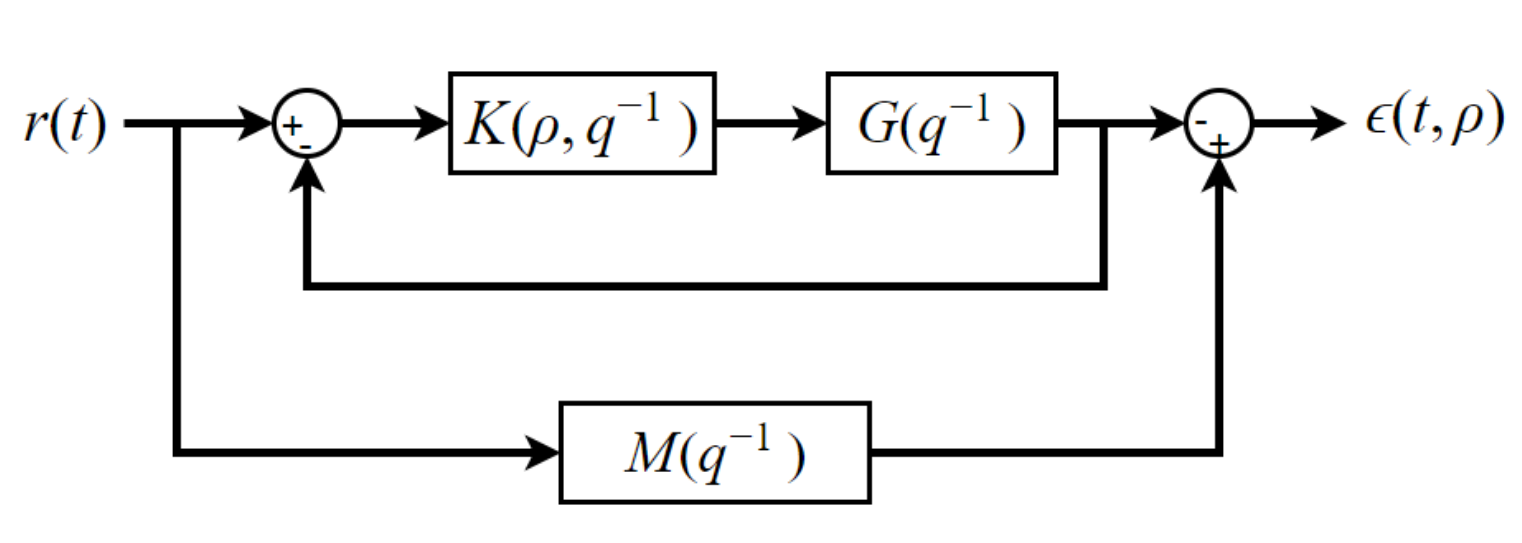
\includegraphics[scale=0.4]{img/DDDC_1.png}
    \caption{Direct Data-Driven Control (DDDC) setting}
    \label{fig:DDDC_setting}
\end{figure}

\begin{quotation}
    \noindent
    \textsf{In the previous chapter we have seen how can we build a model for a dynamical system, linear/nonlinear, SISO/MIMO. For sure, you know that one of the objective of having a mathematical model/description for a given plant is to build a certain \textit{controller} in order to modify the behaviour of the plant itself. In this chapter, going through the description of the \textit{Direct Data-Driven control problem} (DDDC), we will see how to control a certain plant without identify it, but passing directly to the controller design using data.
    }
\end{quotation}

\section{Introduction}
In the field of Control Theory there are mainly three approaches to design a controller for a given plant: 
\begin{enumerate}
    \itemsep-0.2em
    \item \textit{Model-Based technique} in which we have a model for the plant to control, and the problem is solved using some control technique according to the specific problem we have to solve (requirements based, optimal control...);
    \item \textit{Undirect Data-Driven} here since we do not have a model for the plant, at first we retrieve a model  for the plant to be controlled (using some SysId technique), then using the obtained model, some control technique is applied; 
    \item \textit{Direct Data-Driven} Here we have that the controller is designed skipping the plant identification stage, so data are used to build a model directly for the controller.
\end{enumerate}

In particular here the objective, with reference to the \Cref{fig:DDDC_setting} is to design the controller $K$ such that the \textbf{controlled system} could match as well as possible the behaviour of the \textbf{reference model} $M$. In particular given $K(\rho, q^{-1})$, $\rho$ is the \textit{parameter vector} defined as
\begin{equation}
    \rho=[\rho_1 \quad \rho_2 \quad \dots \quad \rho_{n_\rho}]
\end{equation}
\noindent
and we want that 
\begin{equation}\label{eq:approxim}
    T_{ry}(q^{-1})=\frac{G(q^{-1} K(q^{-1}))}{1+G(q^{-1} K(q^{-1}))} \approx 
M(q^{-1})
\end{equation}
Both $K$ and $G$ are assumed to be LTI dynamical systems and the description of $G$ is not available, that is there is no model for the plant to  be controlled. From now on we will assume $M=M(q^{-1})$, $G=G(q^{-1})$ and $K=K(q^{-1})$

\section{Ideal controller $K^*$}
Ideally we want that the \Cref{eq:approxim} could hold with the equality so that
\begin{equation}\label{eq:MMP}
    M=\frac{KG}{1+KG}
\end{equation}
which is the so called \textbf{model matching problem}. We have said that $G$ is not known, but assume for a moment that we are able to know exactly $G$. In this case the model matching problem has a \textit{trivial solution} which corresponds to obtaining an \textbf{ideal controller} $K^*$. By doing simple algebraic manipulation we obtain

\begin{equation}
    M=\frac{GK}{1+GK} \iff M+MGK=GK \iff KG(1-M)=M \iff K^*=\frac{M}{G(1-M)}
\end{equation}
Such a $K^*$ has interesting theoretical property useful in order to go on the description of the DDDC problem, however it can be easily shown that: 
\begin{enumerate}
    \itemsep-0.2em
    \item The resulting $K^*$ from algebraic computations can be \textit{not physically realizable}, using such a trivial formula you are not sure that
    \begin{equation*}
        \deg(D_{K^*}) \ge \deg(N_{K^*}) 
    \end{equation*}
    \item $K^*$ is not guaranteed to provide internal stability of the feedback control system\footnote{
        Remember that an DT LTI Feedback control system is stable if: 
        \begin{itemize}
            \itemsep-0.2em
            \item All of the roots of $1+L(z)$ belongs to the \underline{open unit circle}
            \item No unstable zero-pole cancellations occurs when $L()z$ is formed.
        \end{itemize}
    }, since there can be \textit{unstable zero-pole cancellations}.
\end{enumerate}

\noindent
It can be easily prooved that if we include all of the unstable zeros of $G(q^{-1})$ in the reference model $M(q^{-1})$ then $K^*$ computed is ensuring internal stability of the FCS. But this way you have to pay something: if $M$ (how we will see) is obtained by using some performance requirements, including such new zeros in it will result in a non accurate description of the desired I/O behaviour! We have to derive the controller using a \textbf{different approach}.

\section{Formulation of the DDD control problem}
We wonder here how to solve the model-matching problem when: i) $G(q^{-1})$ is not known, (ii) we can collect I/O data by performing an \textit{open-loop} experiment on the plant to be controlled. Then we want to solve the problem (\ref{eq:MMP}), where $K$ is \textbf{to design}, $G$ is unknown, finally $M$ is given and retrieved taking into account some performance requirements. Going on, you can see that from \Cref{eq:MMP} you can find a \textbf{model matching error transfer function}
\begin{equation}
    E(q^{-1})=M-\frac{KG}{1+KG}
\end{equation}

\noindent
The ideal task is to \textbf{find $K$} such that $E(q^{-1})=0$, we can define the \textbf{output matching error} by multiplying both sides of \Cref{eq:MMP} by the reference $r(k)$
\begin{equation}
    \epsilon(\rho,q^{-1})=\bigg(
        M-\frac{KG}{1+KG}
    \bigg)r(k)
\end{equation}
From this you can see that if $T \approx M$ then $\epsilon(\rho, q^{-1})=0$, and 
\begin{equation}\label{eq:final}
    Mr = \frac{KG}{1+KG}r      \quad    \forall r(k) 
\end{equation}
Here the problem is that we do not have the model $G(q^{-1})$ for the plant and so we cannot find properly the controller $K(\rho, q^{-1})$! How can we go ahead? If we better analyze the \Cref{eq:final} we can exploit a useful insight, in fact
\begin{equation}\label{eq:dddc1}
    Mr-MKGr = KGr \iff (1-M)KGr = Mr \iff KGr(k) = \frac{M}{1-M} r(k)
\end{equation}
Here we have that tber term $Gr(k)$, is by definition equal to the (noise-free) output $y(k)$ of the plant $G$ when you apply the reference signal $r(k)$. The left hand side term is a signal obtained (by simulation) obtained by filtering $r(k)$ by using the transfer function $M/(1-M)$, we can call
\begin{equation}
    s(k)=\frac{M}{1-M}r(k) 
\end{equation}
Then the \Cref{eq:dddc1} can be written as:
\begin{equation}\label{eq:dddc2}
    \Large
    \color{red}
    K(\rho,q^{-1}) y(k) = s(k)
\end{equation}
We can notice that \Cref{eq:dddc2} is formulating a System Identification problem. We want to find $K$, and so its parameters $\rho$ given the input $y(k)$ and the output $s(k)$, where: 
\begin{itemize}
    \itemsep-0.3em
    \item $y(k)$ are the noise free samples of the output of the plant $G$ when the reference signal $r(k)$ is applied as input. Note that since we perform an experiment, we collect noisy data, then you must use
    \begin{equation}
        y(k)=\tilde{y}(k)-\eta(k)
    \end{equation}
    \item $s(k)$ are the samples obtained by stimulating (in simulation) the model $M/(1-M)$ with the reference signal $r(k)$.
\end{itemize}
Finally, we have
\begin{equation}\label{eq:dddc3}
    K(\rho,q^{-1}) [\tilde{y}(k)-\eta(k)] = s(k)
 \end{equation}
that is an \textbf{Input-Error} Set-Membership identification problem where the noise samples are assumed to be UBB (Unknown but bounded), so that
\begin{equation}
    \vert \eta(k) \vert \le \Delta_\eta
\end{equation}

\begin{remark}
    Note that from the development of the theory the following three conditions are equivalent:
    \begin{itemize}
        \itemsep-0.3em
        \item $E(q^{-1})=0$
        \item $\epsilon(\rho,q^{-1})=0$
        \item $K(\rho,q^{-1})r(k)=M (1-M)^{-1} r(k)$
    \end{itemize}
\end{remark}

\section{Set-Membership approach to DDDC (SM-DDDC)}
Now, we have started from the model matching problem, by using some simple algebraic manipulations we have obtained the \textit{output-matching error}, finally we have formulated the problem of designing a controller in the form given by \Cref{eq:dddc3}. Here the objective is to explore how we can formulate a feasible set for the solutions of the problem, and how can be formulated the uncertainty intervals for the parameters describing the controller. It is noticeable that the Input-Error SM-ID problem is a particular case of the Error-In-Variables one! Nothing new, except for the focus we have in this chapter.\\

\noindent
In order to solve the SM-ID problem we need to select the controller class $\mathcal{C}$. For example, this is the same to decide: 
\begin{enumerate}
    \itemsep-0.3em
    \item $\mathcal{C}$=\{class of PID controllers\}
    \item $\mathcal{C}$=\{class of LTI controllers  of fixed and given order $n$\}
\end{enumerate}

How we are going to see in a minute, this framework is providing us a sistematic way to check that the choosen class $\mathcal{C}$ is suitable or not. But first, we introduce also here the equivalent of the feasible parameter set on which is based the SM approach.

\subsection{Feasible Feasible Controller Parameter Set (FCPS)}
Here the parameters that the SM procedure outputs are referred to the controller $K(\rho,q^{-1})$, so we are seeking for a \textbf{Feasible Controller Parameter Set (FCPS)}. In general this can be written as: 
\begin{equation*}
    \begin{aligned}
        \mathcal{D}_\rho=&\{
        \rho\in\mathbb{R}^{n_\rho} \ : s(k)=K(\rho,q^{-1})[\tilde{y}(k)-\eta(k)]\\
        &\vert \eta(k) \vert \le \Delta_\eta \quad k=1,...,N 
    \}
    \end{aligned}
\end{equation*}
In order to give an example we can assume that $\mathcal{C}=\{\text{class of first order LTI controllers}\}$, in this way we have a closed form for $K(\rho,q^{-1})$:
\begin{equation}
    K(\rho,q^{-1})=\frac{\rho_2+\rho_3q^{-1}}{1+\rho_1 q^{-1}}
\end{equation}
In this way the FCPS becomes ($n_\rho=3$): 
\begin{equation}
    \begin{aligned}
        \mathcal{D}_\rho=&\{
        \rho\in\mathbb{R}^3: s(k) + \rho_1 s(k-1) -\rho_2 \tilde{y}(k)\\
        &-\rho_3 \tilde{y}(k-1) + \rho_2 \eta(k) + \rho_3 \eta(k-1)=0 \quad k=2,...,N\\
        &\vert \eta(k) \vert \le \Delta_\eta \quad k=1,...,N
    \}
    \end{aligned}
\end{equation}

We know that there is no way to eliminate the dependence on the noise samples $\eta(k)$, fir this reason we have to extend the FCPS into an \textit{Extended Feasible Controller Parameter Set} (EFCPS) $\mathcal{D}_{\rho,\eta}$, defined by: 

\begin{equation}
    \begin{aligned}
        \mathcal{D}_{\rho,\eta}=&\{
        \rho\in\mathbb{R}^3, \ \eta \in \mathbb{R}^N: s(k) + \rho_1 s(k-1) -\rho_2 \tilde{y}(k)\\
        &-\rho_3 \tilde{y}(k-1) + \rho_2 \eta(k) + \rho_3 \eta(k-1)=0 \quad k=2,...,N\\
        &\vert \eta(k) \vert \le \Delta_\eta \quad k=1,...,N
    \}
    \end{aligned}
\end{equation}

If at this stage $\mathcal{D}_{\rho,\eta}$ is \textbf{empty} than, there is no controller in the considered class $\mathcal{C}$ which solves the control problem. This is an evidence that the EFCPS is giving us a tool by which we can check if we have correctly chosen the controller class. \\
Moreover, it holds that $\mathcal{D}_{\rho, \theta}=\varnothing $ if and only if at least one of the POP to be solved for computing the \textbf{Controller Parameter Uncertainty Intervals (CPUIs)} has \texttt{exitflag}<0. 

\subsection{Summarizing the $K(\rho,q^{-1})$ design procedure}
In order to \textbf{design a Direct Data-Driven controller (DDDC)} $K(\rho,q^{-1})$: 
\begin{enumerate}
    \itemsep-0.3em
    \item Perform an open-loop experiment by applying $r(k)$ to the plant to be controlled and collect the output $\tilde{y(k)}=y(k)+\eta(k)$, with $\eta(k)$ bounded; 
    \item Build the Feasible Controller Parameter set and Extended Feasible Controller Parameter Set ($\mathcal{D}_{\rho}$ and $\mathcal{D}_{\rho,\eta}$).
    \item Compute the \textit{Controller Parameter Uncertainty Intervals}:
    \begin{equation}
        CPUI_{\rho_i}=[\underline{\rho}_i, \overline{\rho}_i] \quad 
        \underline{\rho}_i= \min_{\rho,\eta \in \mathcal{D}_{\rho,\eta}} \rho_i \quad
        \overline{\rho}_i= \max_{\rho,\eta \in \mathcal{D}_{\rho,\eta}} \rho_i 
    \end{equation}
    \item Two sitautions can occur at this point:
    \vspace{-0.3cm}
    \begin{itemize}
        \itemsep-0.3em
        \item[a] If one of the problem is infeasible than update $\mathcal{C}$;
        \item[b] If all the POPs are feasible (\texttt{exitflag}>0) we obtain the CPUIs for all $rho_i$
    \end{itemize}
    \item Build the controller transfer function as:
    \begin{equation}
        K_c(\rho^c,q^{-1})=\frac{\rho^c_{n+1} + \rho^c_{n+2}q^{-1}+...+\rho^c_{2n+1} q^{-n}}
        {1+\rho_1^c q^{-1}+...+\rho_n^c q^{-n}}
    \end{equation}
    where
    \begin{equation}
        \rho^c =[\rho^c_1,..., \rho^c_{2n+1}] \iff \rho_i^c = \frac{\underline{\rho}_i+\overline{\rho}_i}{2}
    \end{equation}
    \noindent
    If $K^c$ belongs to $\mathcal{C}$, then the ideal controller belongs to the Feasible Controller Set
\end{enumerate}

\begin{remark}
    It can be prooved that the central estimate $\rho^c$ is the solution to the following optimization problem
    \begin{equation}
        \rho^c = \arg \min_{\rho\in\mathbb{R}^p} \max_{\rho'\in\mathcal{D}_{\rho}} {
            \Vert \rho-\rho'\Vert_\infty
        }
    \end{equation}
    this is called the \textbf{Chebychev center in the $\ell_\infty$-norm} and it is the point of minimum distance from the farthest point in the FCPS. Then this is the point guaranteeing the \textit{minimum uncertainty} which is possible.
\end{remark}

\section{Stability Guarantee in SM-DDDC}





